\documentclass{article}
\usepackage[margin=1in]{geometry}
\usepackage{amsmath, amssymb, amsthm}
\usepackage{enumitem}

% colored links
\usepackage{hyperref}
\hypersetup{
    colorlinks=true,
    linkcolor=blue,
    filecolor=magenta,      
    urlcolor=blue,
    }



% Inputting Python code
\usepackage[dvipsnames]{xcolor}
\definecolor{textblue}{rgb}{.2,.2,.7}
\definecolor{textred}{rgb}{0.54,0,0}
\definecolor{textgreen}{rgb}{0,0.43,0}
\usepackage{upquote}
\usepackage{listings}
\lstset{
    language=Python, 
    tabsize=4,
    basicstyle={\ttfamily},
    keywordstyle=\color{textblue},
    commentstyle=\color{textgreen},
    stringstyle=\color{textred},
    frame=none,
    columns=fullflexible,
    keepspaces=true,
    showstringspaces=false,
    xleftmargin=-15mm, % manual adjustment, figure out permanent solution
}
\usepackage{tcolorbox}
\tcbuselibrary{skins,hooks}
\usetikzlibrary{shadows}
\usepackage{lipsum}


%Images
\usepackage{graphicx}
    \usepackage{subcaption}
    \usepackage{float}
    \newcommand{\glass}{
\includegraphics[height=4ex]{images/glass.png}}
    \newcommand{\rum}{
\includegraphics[height=4ex]{images/rum.png}}
    \newcommand{\mixedrum}{
\includegraphics[height=4ex]{images/mixed_rum.png}}
    \newcommand{\pineapple}{
\includegraphics[height=4ex]{images/pineapple.png}}
    \newcommand{\pinacolada}{
\includegraphics[height=4ex]{images/pina_colada.png}}
    \newcommand{\mixedpineapple}{
\includegraphics[height=4ex]{images/mixed_pineapple.png}}
    \newcommand{\coconut}{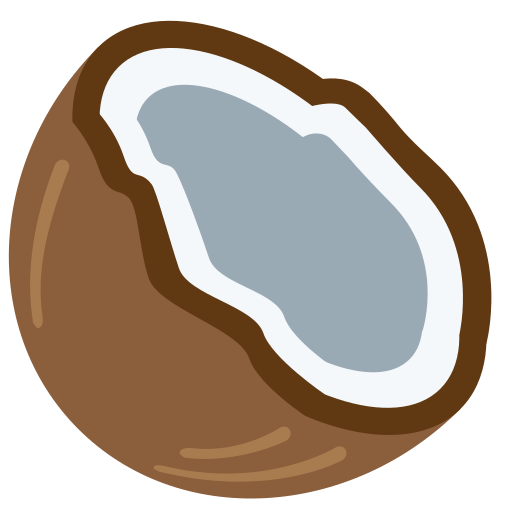
\includegraphics[height=4ex]{images/coconut.png}}
    \newcommand{\juice}{\includegraphics[height=4ex]{images/juice.png}}
    \newcommand{\heart}{
\includegraphics[height=4ex]{images/heart.png}}
    


%Formatting and Spacing
\setitemize[1]{noitemsep, parsep = 5pt, topsep = 5pt}
\setenumerate[1]{label = (\alph*), parsep = 1pt, topsep = 5pt}
\setlength\parindent{0pt}
\linespread{1.1}

% title
\title{\vspace{-1cm}CS 2051: Honors Discrete Mathematics \\Spring 2023 Homework 7 Supplement outline}
\author{Sarthak Mohanty, \tiny{Anant Gupta} }
\date{}

\begin{document}

\maketitle

% to do: fix titles
Title: ECC is the new RSA
\section*{Overview}

Over the past few weeks, we've covered number theory, as well as a nice application of it through the use of RSA cryptography.

\vspace{2mm}
Elliptic Curve Cryptography (ECC) is one of the most powerful cryptosystems in use today. Companies are using ECC everything to secure everything from our customers' HTTPS connections to how we pass data between our data centers. In fact, based on currently understood mathematics, ECC provides a significantly more secure foundation than first generation public key cryptography systems like RSA, for reasons we'll explore in detail later. The specific implementations you might learn in this supplement aren't as important as the general framework, understanding, and ideas you'll develop.

\vspace{2mm}
\textbf{Note.} As I was making this assignment, I stumbled across \href{https://andrea.corbellini.name/2015/05/17/elliptic-curve-cryptography-a-gentle-introduction/}{this} excellent blog post, and realized it covers some of these concepts a lot better than I ever could. For this reason, some of the exposition is adapted from this resource.


\section*{Cryptography Primer}
    Before we continue, it is beneficial to take a step back, and discuss cryptography as a whole.

\subsection*{Symmetric vs Asymmetric Systems}

    In cryptography, there are two main types of encryption algorithms: symmetric and asymmetric. 

    \vspace{3mm}
    \textbf{Symmetric, or private-key, encryption} uses the same key to both encrypt and decrypt the message. Symmetric encryption algorithms are generally faster and more efficient, but they require the sender and the recipient to share a secret key. The most prominent example is the AES cipher.\footnote{some of your classmates have chosen this as their group project!} 

    \vspace{3mm}
    On the other hand, \textbf{asymmetric, or public-key encryption} algorithms are slower and less efficient, but they allow the sender to send a message securely to the recipient without sharing a secret key. Examples include RSA, Diffie-Helman, and ECCDH.

\subsection*{Trapdoor Functions}
    
    Trapdoor functions are an essential component of asymmetric encryption algorithms. A trapdoor function is a function that is easy to compute in one direction, but difficult to compute in the opposite direction without knowledge of additional information, such as a secret key.
    
    \vspace{2mm}
    As an example, the trapdoor function in RSA encryption is the modular exponentiation function, $c = m^e \mod N$, where $m$ is the plaintext, $e$ is the public exponent, $N$ is the modulus and $c$ is the ciphertext. The trapdoor information is the private key, which consists of the factors of $N$. In the opposite direction, decryption is performed by computing $m = c^d \mod N$, where $d$ is the private exponent derived from the private key.


\section*{Part 1: Diffie-Helman}

\subsection*{Diffie-Hellman Key Exchange}

The Diffie-Hellman key exchange is a cryptographic protocol that allows two parties to generate a shared secret key over an insecure communication channel. The protocol is named after its inventors, Whitfield Diffie and Martin Hellman. There is a classic analogy for the DH key exchange, which we presnt below:
\begin{tcolorbox}
    Professor Brito and Lianet (Brito’s wife!) have a famous Piña Colada recipe that they keep secret from the rest of the world. It is so secret in fact, that neither Brito nor Lianet know the full parts of the recipe! However, using their knowledge on how the Diffie-Helman key exchange algorithm works, they have devised a unique way of making the drink.

    \vspace{2mm}
    To make their famous Piña Colada, Brito and Lianet have their own secret ingredients, which they mix separately. Brito mixes a secret amount of rum to a glass, while Lianet mixes a secret amount of pineapple juice to another glass. These individual mixtures represent the private keys of each party:

    $$\text{Brito:} \glass + \coconut + \rum = \mixedrum \quad \text{Lianet:} \glass + \coconut + \pineapple = \mixedpineapple$$
    
    \vspace{2mm}
    Next, they swap glasses. This represents the public key exchange. Note that because the ingredients were mixed in, it is very difficult for either Brito or Lianet to determine the exact contents of the current glass.

    $$\text{Brito: \mixedpineapple \quad Lianet: \mixedrum}$$
    
    Once they have exchanged their public keys, they each use their own private key to mix with the other party's public key to generate a shared secret key, in this case the final drink.

    $$\text{Brito:} \mixedpineapple + \rum = \pinacolada \quad \text{Lianet:} \mixedrum + \pineapple = \pinacolada$$

    \vspace{2mm}
     This shared secret key can be used to establish a secure communication channel, just like the delicious Piña Colada they created together.
     % $$\text{Brito}\quad\heart\quad\text{Lianet}$$
\end{tcolorbox}
    In this analogy, the rum and pineapple juice represent the private keys, while the remaining ingredients represent the public key exchange. The shared secret key is the final product, which can be used for secure communication between the two parties.


    \vspace{2mm}
    See the textbook for actual diffie-helman.

\subsection*{Trapdoor Function: Discrete Log Problem}



\subsection*{Attacks}

\begin{center}
    \textbf{Brute Force}
\end{center}

All public key schemes are in theory susceptible to a brute force attack. Try all possible values. This takes $\mathcal{O}(n)$ time.

\begin{center}
    \textbf{Baby-Step Giant-Step algorithm}
\end{center}

This algorithm trades off space to improve the running time over brute force. The idea is to write $x = i\lceil n \rceil + j$ for $0 \le i,j \le \lceil n \rceil$. For simplicity let $m = \lceil n \rceil$. First compute $g^j$ for all $0 \le j \le m$. Then we compute $y\cdot g^{-im}$ for each $0 \le i \le m$. Notice that both can be done in $O(\sqrt n )$ time. If we could find a collision $y\cdot g^{-im} = g^j$, then $x = im + j$. To find this collision efficiently we store all $g^j$ (for all $0 \le j \le m$) by hash-sets and when we compute $y\cdot g^{-im}$ we simply check if that value is already present in the set. This finds the collision in $O(\sqrt{n})$ time (as we need to check if the value is present in the set only $O(\sqrt{n})$ times). Overall this algorithm uses $O(\sqrt{n})$ space and time.

% \begin{center}
%     \textbf{Pollard rho algorithm}
% \end{center}


% This is a randomized algorithm that works in $O(\sqrt{n})$ expected time and with $O(1)$ space requirement. We descirbe the algorithm for prime modulus. All the operations described in this section work mod $p$.

% The idea is to divide $\{1, \dots n-1\}$, which are the possible $x$s into three sets, say, $S_0, S_1$ and $S_2$ of roughly equal size. In practice we do it by taking $x \pmod 3$ ie. $x \in S_i$, where $i = x \pmod 3$. We do a random walk starting at $x_0 = g^{a_0} y^{b_0}$ where $a_0 = b_0 = 0$. To generate $x_{i+1}$ from $x_i$ we follow the following rule:

% \begin{equation*}
%     x_{i+1} = 
%     \begin{cases}
%         x_i^2 \text{ if } x_i \in S_0 \\
%         yx_i \text{ if } x_i \in S_1 \\
%         gx_i \text{ if } x_i \in S_2
%     \end{cases}
% \end{equation*}

% Corresponding to these $x_i$'s we also maintain the $a_i, b_i$ such that $x_i = g^{a_i} y^{b_i}$. Now suppose we find $i$ and $j$, $i \neq j$, such that $x_i = x_j$, or $g^{a_i} y^{b_i} = g^{a_j} y^{b_j}$. Then $g^{a_i - a_j} = y^{b_j - b_i} \pmod n$. Substituting $y = g^x$, we get the equation $a_i - a_j = x (b_j - b_i)$. We then solve this using a linear congruence solver to obtain $x$.

% So all we need to so now is to find $i$ and $j$, $i \neq j$, such that $x_i = x_j$. This is done using the classic Floyd's Hare and Tortoise algorithm (by which the algorithm gets the $\rho$ in its name). Essentially there are two pointers, one that jumps two steps and another that jumps only one. If there are $i$ and $j$, such that $x_i = x_j$, then these pointers would meet at the same point, giving us $i$ and $j$.

\begin{center}
\textbf{General Number Field Sieve (GNFS)}
\end{center}

The General Number Field Sieve is a factorization algorithm that is particularly efficient for numbers with large prime factors. The implementation It is a multi-step process that involves finding a smooth polynomial and then finding the roots of that polynomial.

\vspace{2mm}
It first selects a sequence of integers that has a high probability of containing a factor of the number being factored. It then tries to find smooth numbers in this sequence, which are numbers whose prime factors are all below a certain bound. Finally, it uses linear algebra to combine these smooth numbers in a way that allows it to extract non-trivial factors of the number being factored. GNFS is one of the most efficient known factorization algorithms for large integers.

% add reference for source
\vspace{2mm}
There is one final important note about factoring algorithms such as the general number field sieve. Such algorithms get more efficient as the size of the numbers being factored get larger. The gap between the difficulty of factoring large numbers and multiplying large numbers is shrinking as the number (i.e. the key's bit length) gets larger. As the resources available to decrypt numbers increase, the size of the keys need to grow even faster. This is not a sustainable situation for mobile and low-powered devices that have limited computational power. The gap between factoring and multiplying is not sustainable in the long term.

\vspace{2mm}
All this means is that RSA is not the ideal system for the future of cryptography. In an ideal Trapdoor Function, the easy way and the hard way get harder at the same rate with respect to the size of the numbers in question. We need a public key system based on a better Trapdoor. In 1985, such a system was found, revolving around an (then) arcane field known as elliptic curves.

\begin{tcolorbox}
% [colback=yellow!30]
    In this part, you'll fully implement the Diffie-Helman key exchange and try to break it on small numbers.

    Class Actor:
    \begin{itemize}
        \item \lstinline{computePublicKey(self)}: See docs for details
        \item \lstinline{computeSecret(self, offer)}: See docs for details
    \end{itemize}

    Class BadActor
    \begin{itemize}
        \item \lstinline{brute(self, g, y, n):}: This function takes in the parameters for the discrete log problem, and returns the correct answer using brute force.
        \item \lstinline{bsgs(self, g, y, p)}: Same thing as above, but with baby-step giant-step algorithm.
    \end{itemize}
\end{tcolorbox}



\section*{Part 2: Enter Elliptic Curves}

The standard form for an elliptic curve is $$y^{2} = x^{3} + Ax + B,$$ where $A$ and $B$ are constants.  This will be referred to as the Weierstrass equation for an elliptic curve. For reasons that will be discussed later, also include the point $\{\infty\}$ in this function.

\subsection*{The Group Law}
    One important aspect of elliptic curves is that we can start with two points, or even one point on an elliptic curve, and produce another point.


\begin{figure}[htbp]
    \centering
    
    \begin{subfigure}[t]{.45\textwidth}
        \centering
        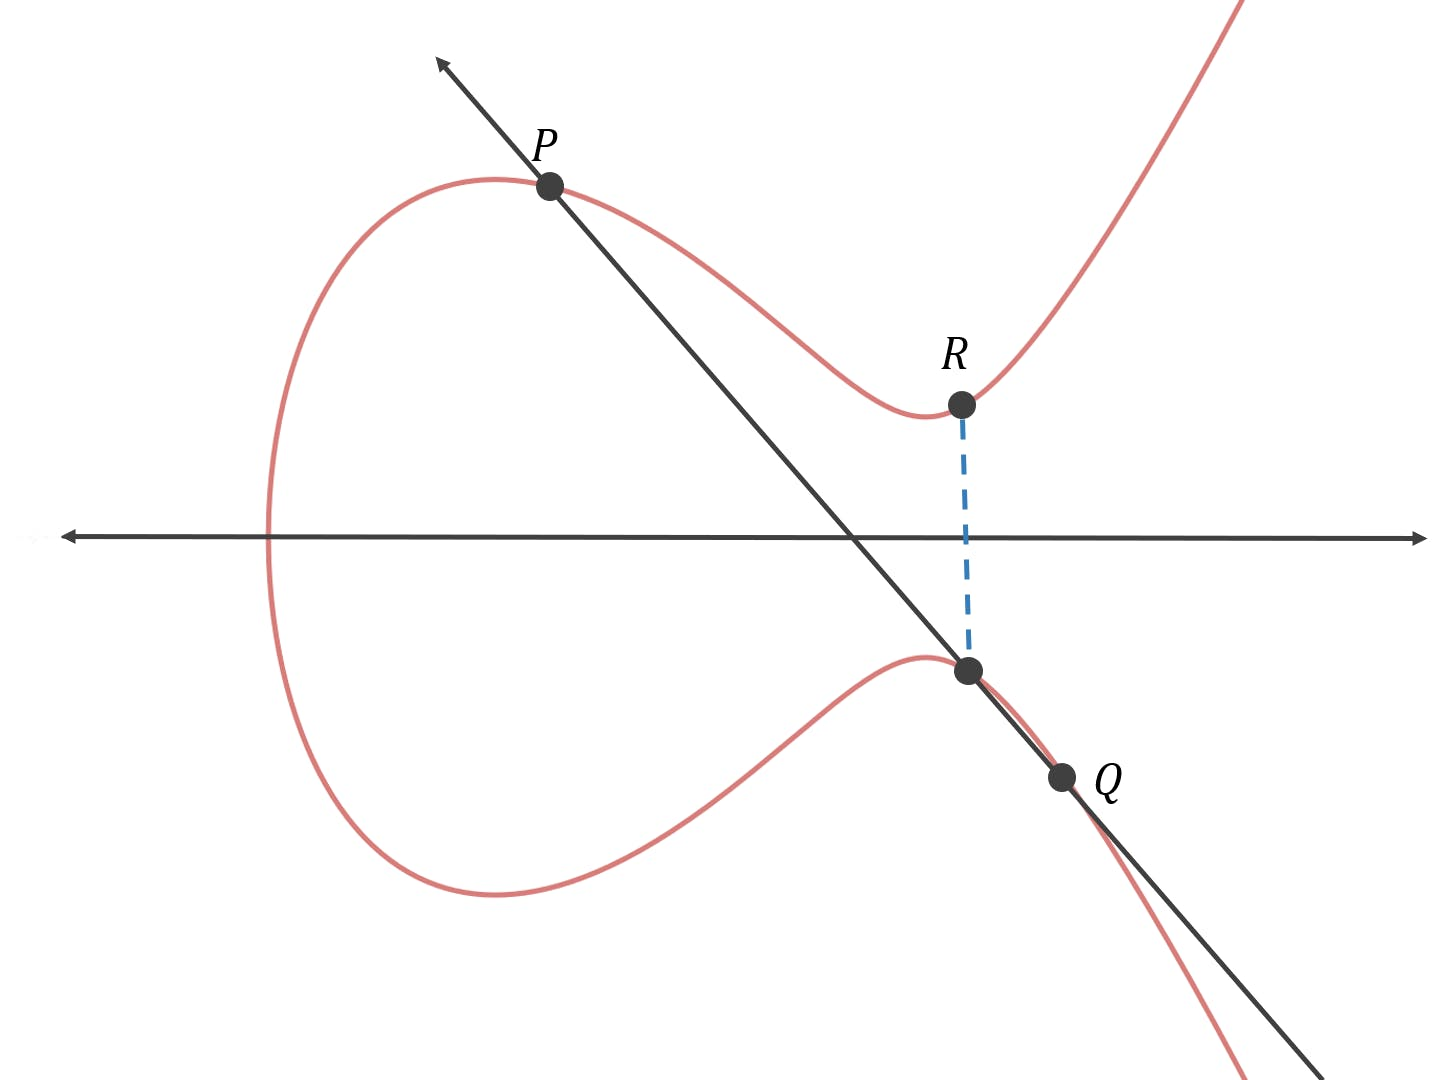
\includegraphics[scale = 0.15]{images/point_addition.jpeg}
        \caption{Point Addition}
        \label{fig:point_addition}
    \end{subfigure}
    \begin{subfigure}[t]{.45\textwidth}
        \centering
        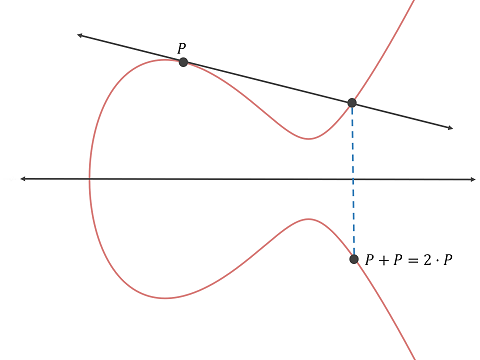
\includegraphics[scale = 0.8]{images/point_scalar_multiplication.png}
        \caption{Point scalar multiplication}
        \label{fig:point_multiplication}
    \end{subfigure}
    \caption{Group law visualized.}
    \label{fig:edge_case}
\end{figure}


\begin{tcolorbox}
    In this part, you'll implement point addition and point multiplication on elliptic curves

    
    \textbf{In this part, you'll implement the following functions:}
    \begin{itemize}
        \item \lstinline{point_addition(elliptic_curve, P, Q)}: This function takes in an elliptic curve 
        \item \lstinline{point_scalar_multiplication(elliptic_curve, k, P))}: This function takes in an elliptic curve of the form described, a scalar integer $k$, and a point $P$, and repeatedly multiplies this result to output a number.
    \end{itemize}
    You can run \lstinline{visualize_addition} and \lstinline{visualize_multiplication} to generate the corresponding visualizations mentioned above. If you want more examples, there's an interactive tool \href{https://andrea.corbellini.name/ecc/interactive/reals-add.html}{here}
    Notes: This part is just algebra and geometry. Since I know it's been a while since many of you touched this, here's a few steps you get you started.
    \begin{itemize}
        \item For point addition, we assumed that $P \ne Q \ne \infty$. For this reason, we can draw the line $L$ through $P_{1}$ and $P_{2}$. Its slope is $$m = \frac{y_{2} - y_{1}}{x_{2} - x_{1}}.$$ If $x_{1} = x_{2}$, then $L$ is vertical, so the resulting point is just $\infty$. Now let's assume that $x_{1} \ne x_{2}$. The equation of $L$ is then $$y = m(x - x_{1}) + y_{2}.$$ To find the intersection of this line with the elliptic curve, we can substitute the above equation into the formula for an elliptic curve $$y^{2} = x^{3} + ax + b.$$ Finally, we can reflect the above point across the $x$-axis to obtain the point $P_{3} = (x_{3}, y_{3})$.
        \item For point scalar multiplication, we have that $P = Q = (x_{1}, y_{1})$. When two points on a curve are very close to each other, the line through them approximates a tangent line. Therefore, when the two points coincide, we take the line $L$ through them to be the tangent tine. Implicit differentiation allows us to find the slope $m$ of $L$: $$2y \frac{dy}{dx} = 3x^{2} + A,\text{\quad so\quad} m = \frac{dy}{dx}\frac{3x_{1}^{2} + A}{2y_{1}}.$$ If $y_{1} = 0$ then the line is vertical and we set $P_{1} + P_{2} = \infty$, as before. Otherwise, we plug in values and solve as before.
    \end{itemize}
    
\end{tcolorbox}

\section*{Part 3: In The Field}
The elliptic curve cryptography (ECC) uses elliptic curves over the finite field $\mathbb{F}_{p}$ (where $p$ is prime and $p > 3$). For example, the ``Bitcoin curve" secp256k1 takes the form:
$$y^{2} \equiv x^{3} + 7 \pmod{p}$$


The group law over $\mathbb{F}_{p}$ is similar, but not identical to in the field of real numbers. It is stated (and proven) in \href{https://arxiv.org/pdf/1710.00214.pdf}{this} research paper.


\begin{tcolorbox}
    In this part, you'll visualize elliptic curves over finite fields, as well as implement point addition and point multiplication over these fields

    
    \textbf{In this part, you'll implement the following functions:}
    \begin{itemize}
        \item \lstinline{generate_point_cloud(a, b, p)}: This takes in an elliptic curve and returns a set of all valid points in the curve over that field. See docs for example.
        \item \lstinline{point_addition(P, Q, a, b, p)}: This function takes in an elliptic curve and two points, and adds them.
        \item \lstinline{point_scalar_multiplication(P, n, a, b, p)}: This function takes in an elliptic curve of the form described, a scalar integer $k$, and a point $P$.
    \end{itemize}
    
\end{tcolorbox}

\section*{Part 4: ECC in Action: Elliptic-curve Diffie Helman}

% You've devleoped some undrestanding of how elliptic curves work, but it's naturarl to doubt the connection between them. This is where yopu're wrong. Note that... this is called \textit{order independence}. This makes it really easy to modify diffie helman to accomodate our elliptic curves, as follows:

% This order independence also makes it easy to see why ECC takes less storage space than Diffie-Helman, 

\subsection*{The Elliptic-curve Discrete Log Function}



    \vspace{3mm}
    Trapdoor function in Elliptic Curve Cryptography (ECC). In ECC, the trapdoor function is the scalar multiplication operation $Q = kP$, where $P$ is a point on the elliptic curve, $k$ is the scalar and $Q$ is the result of the scalar multiplication. The trapdoor information is the private key, which is the scalar $k$. Decryption is performed by computing $Q = -kP$.


For carefully chosen (by cryptographers) finite fields and elliptic curves, the ECDLP problem has no efficient solution.

The multiplication of elliptic curve points in the group $\mathbb{F}_{p}$ is similar to exponentiation of integers in the group $\mathbb{Z}_{p}$ (this is known as multiplicative notation) and this is how the ECDLP problem is similar to the DLP problem (discrete logarithm problem).

See \href{https://www.youtube.com/watch?v=gAtBM06xwaw}{this} video for implementation details

\begin{tcolorbox}
% [colback=yellow!30]
    In this part, you'll implement a elliptic-curve diffie helman key exchange and try to break it on small numbers. You should directly call the methods you constructed in Part 2. You should replicate the methods you created in Part 1, this time accommodating for the elliptic-curve element.

    Class Actor:
    \begin{itemize}
        \item \lstinline{computePublicKey(self)}: See docs for details
        \item \lstinline{computeSecret(self, offer)}: See docs for details
    \end{itemize}

    Class BadActor
    \begin{itemize}
        \item \lstinline{brute(self, g, y, n):}: This function takes in the parameters for the discrete log problem, and returns the correct answer using brute force.
        \item \lstinline{bsgs(self, g, y, p)}: Same thing as above, but with baby-step giant-step algorithm.
    \end{itemize}
\end{tcolorbox}


% https://arstechnica.com/information-technology/2015/11/op-ed-how-did-they-break-diffie-hellman/?comments=1&comments-page=1#comment-30128933

\subsection*{Conclusion}

    \subsubsection*{RSA vs ECC}

    Since RSA and ECC essentially serve the same purpose, there have been many heated discussions as to which implentation to use. The main pro of using ECC is the fact that it uses fewer memory and CPU resources, important as mobile computing becomes more ubiquitous. However, there are a few flaws with ECC. First, there are only a few curves that work and the NIST is in contorl of most of them, but people distrust NIST. Second, 

    \vspace{2mm}
    Finally, neither ECC nor RSA are secure against quantum computers. 



    \subsubsection*{Real World Application}

    Even with all those downsides, more and more companies are using ECC, including

    \begin{center}
        Amazon, Bing, Dropbox, Facebook, Flickr, GitHub, Instagram, \\
        LinkedIn, MSN, Netflix, Pinterest, PirateBay, Quora, Snapchat, \\
        SoundCloud, Spotify, StackOverflow, Tumblr, Twitter, Uber, \\
        Vimeo, Vine, Yahoo, Yelp, YouTube, Wikipedia, Wordpress,\dots
    \end{center}

Two prominent examples:
    \begin{itemize}
        \item \href{https://chat.openai.com/chat}{ChatGPT}
        \item \href{https://proton.me/blog/elliptic-curve-cryptography}{ProtonVPN}
    \end{itemize}

    to do: explain how you can see ecc implentation on website. Click on lock on top left of website, click on ``connection is secure", click on ``certificate is valid", you should see ECC used for certificate

    
    assymetric not often used since takes long time. Instead, key exchange is done using assymetric andthen symmetric is used to send the actual messages, as can be seen \href{https://github.com/nakov/Practical-Cryptography-for-Developers-Book/blob/master/asymmetric-key-ciphers/ecc-encryption-decryption.md}{here}


\section*{Submission Instructions (10 pts)}
    After you fill the appropriate functions, submit the following files to Gradescope and make sure you pass all test cases:
    \begin{itemize}
        \item \lstinline{diffie_helman.py}
        \item \lstinline{elliptic_curves.py}
        \item \lstinline{ECDH.py}
    \end{itemize}

    \vspace{3mm}
    \textbf{Notes}
    \begin{itemize}
        \item The autograder may not reflect your final grade on the assignment. We reserve the right to run additional tests during grading.
        \item Do not import additional packages, as your submission may not pass the test cases or manual review.
    \end{itemize}

    
    % These factoring algorithms get more efficient as the size of the numbers being factored get larger. The gap between the difficulty of factoring large numbers and multiplying large numbers is shrinking as the number (i.e. the key's bit length) gets larger. As the resources available to decrypt numbers increase, the size of the keys need to grow even faster. This is not a sustainable situation for mobile and low-powered devices that have limited computational power. The gap between factoring and multiplying is not sustainable in the long term.

\section*{References}

\begin{itemize}
    \item explanation for group law name is \href{https://www.math.brown.edu/reschwar/M1540B/elliptic.pdf}{here}
    \item why infinity is added \href{https://crypto.stackexchange.com/questions/70507/in-elliptic-curve-what-does-the-point-at-infinity-look-like}{here}
    \item This (heavy) textbook is a good resource if you want to explore the mathematics of elliptic curves in further detail.
\end{itemize}


\end{document}